\chapter{计算机病毒}

我们定义计算机“病毒”为一个程序,它可以复制自身来调整自己从而感染其他程序。通过感染特性,病毒可以通过计算机系统或者网络进行广泛传播,使用每一个用户的授权来感染他们的程序。每一个被感染的程序也可能会表现为病毒,从而使得感染扩散。


接下来的伪程序展示了一个病毒如何写成一个伪计算机语言。符号‘:=’表示定义,符号‘:’标注一个状态,符号‘;’用于分隔状态,符号‘=’用于赋值或者比较,符号‘~’表示否,符号‘{’和‘}’将状态序列放在一起,符号‘…’表示代码的不相关部分已经略去了。


示例病毒(V)(图\ref{fig1})通过搜寻没有“1234567”开头的可执行文件来寻找一种不可感染可执行文件(E),将V加入E,将它变成一个感染文件(I)。然后V检查一些触发条件和破坏是否是正确的。最后,V执行剩余的前缀程序。当用户尝试执行E,那么I会在它的部分执行;它会感染其他的文件并且把它当做E来执行。由于感染的轻微延迟异常,I在触发条件导致破坏之前被看做是E。我们注意到,病毒不需要预先考虑自己,也不会限制于每次使用的单个感染。

%%% 图1

\begin{figure}[h!]
    \centering
    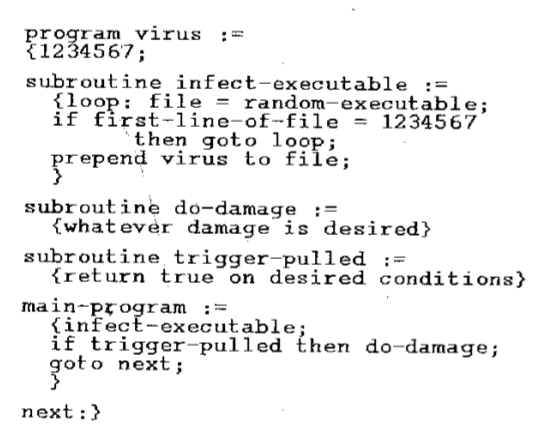
\includegraphics[width=0.60\textwidth]{figure/fig1.png}
    \caption{Simple Virus V} 
    \label{fig1}
\end{figure} 


病毒的一个常见的误解是它的程序简单地通过网络传播。蠕虫程序,“核心战争”,和其他类似的项目做到这一点,但实际上没有人涉及到感染的部分。病毒的关键特性是它感染其他程序的能力,从而达到共享用户之间的传递闭包。例如,如果V感染用户的一个可执行文件(E),然后用户B也运行 E,那么V可能蔓延至用户B的文件。


应该指出,病毒不可以用于邪恶的目的或
者是成为一个木马。例如,一个压缩病毒可以写来
用于找到未受感染的可执行文件,在用户许可
的情况下压缩它们,并且预先考虑自己而非
它们。在执行时,受感染的程序进行解压,然后
正常执行。因为它总是在执行服务之前寻
求允许,所以这不是一个木马,但
因为它有感染特性,所以它仍然是一个病毒。研究
表明,在平均系统中,这种病毒可能节省由
可执行文件占据的超过50\%的空间。被感染
的程序的表现将下降,这是因为它们被解压了,
从而压缩病毒实现一个特定的时间与空
间的权衡。病毒样本压缩可以编写如下,见图\ref{fig2}。

\begin{figure}[h!]
    \centering
    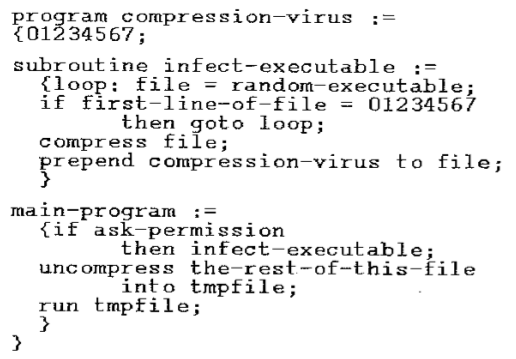
\includegraphics[width=0.60\textwidth]{figure/fig2.png}
    \caption{Compression Virus C} 
    \label{fig2}
\end{figure} 
%%%%图2

这个程序(C)找到了一个未感染可执行文件(E),压缩它,并且突出显示C形成一个感染可执行文件(I)。然后将剩余的自己解压为一个临时文件并且可以正常执行。当运行I时,在将I解压成一个临时文件盒执行之前,它会寻找并压缩其他可执行文件。传播的效果是通过系统压缩可执行文件,并解压它们进行执行。用户将有重大延迟,因为他们的可执行文件是在解压后才运行的。


一个更具威胁性的例子中,我们假设通过以下的方法修改程序V,一是指定在一个给定的数据和时间进行触发,二是指定通过无限循环的方式进行破坏。在大多数现代系统的共享水平下,整个系统可能无法在指定的日期和时间条件下使用。可能需要大量的工作来消除这种病毒的破坏。
这一修改如图\ref{fig3}所示。

\begin{figure}[h!]
    \centering
    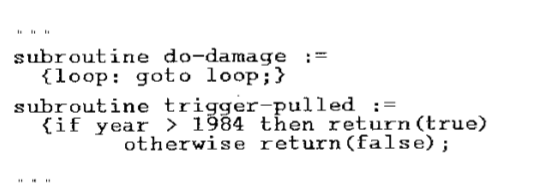
\includegraphics[width=0.60\textwidth]{figure/fig3.png}
    \caption{A denial of services virus} 
    \label{fig3}
\end{figure} 
%%%%图3

作为计算机病毒的一个类比,可以考虑一个可以
100\%感染的生物疾病,
每当动物交流时就会传播,在给定的时刻立即杀死所有被感染的动物,并且在那个时刻之前没有检测到副作用。如果疾病的引入和见效之间存在一周的延迟,将很有可能只有少数偏远村庄能够幸存,并肯定会消灭绝大多数的现代社会。如果类似于这种类型的电脑病毒可以传遍世界所有的计算机,它可能会在很长的时间阻止大多数电脑的使用,并且在现代政府、金融、商业和学术机构中造成很大的破坏。




